% 图 7.9 (a) 闭合费面腰部闭合轨道 + 法向 v(k) 箭头 + B (b) 开放轨道波纹面片 + B⊙
\documentclass[tikz,border=5pt]{standalone}
\usetikzlibrary{arrows.meta,decorations.pathmorphing}
\usepackage{amsmath}
\usepackage{bm}
\usepackage{fontspec}
\setmainfont{Times New Roman}
\begin{document}
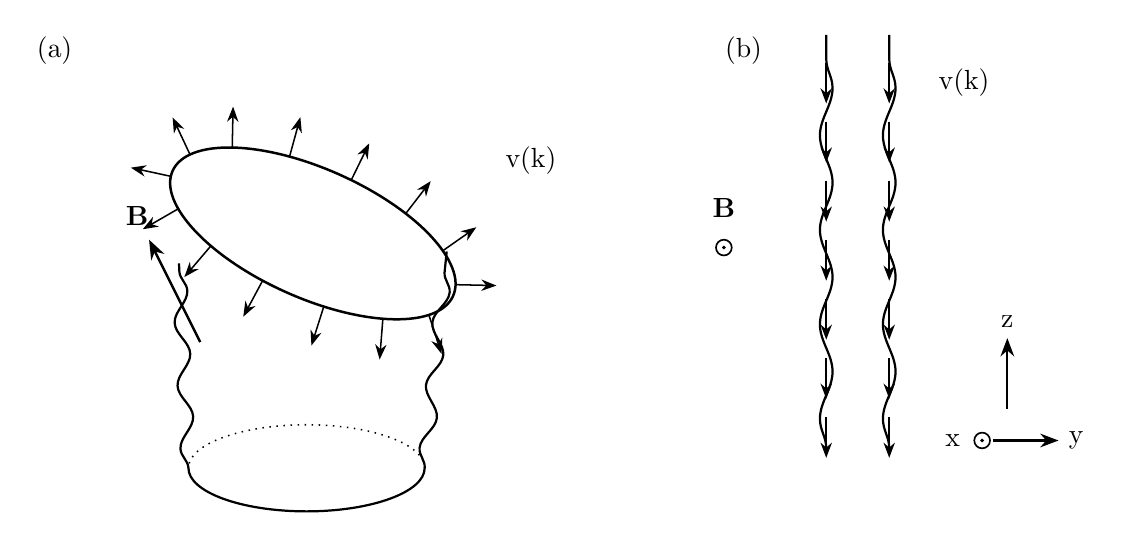
\begin{tikzpicture}[line width=0.8pt,>=Stealth]
% ---------- (a) 闭合费面 ----------
\begin{scope}
\node at (-3.2,5.3) {(a)};
% 底部椭圆：前面实线，后面点线
\draw[dotted,line width=0.55pt] (1.5,0) arc (0:180:1.5 and 0.55);
\draw (-1.5,0) arc (180:360:1.5 and 0.55);
% 波纹侧面
\draw[decorate,decoration={snake,amplitude=0.9mm,segment length=8mm,
  post length=0mm}] (-1.5,0) -- (-1.62,2.6);
\draw[decorate,decoration={snake,amplitude=0.9mm,segment length=8mm}] (1.5,0) -- (1.78,2.75);
% 顶部椭圆（闭合轨道，倾斜）
\begin{scope}[rotate around={-24:(0.08,2.98)}]
  \draw[line width=0.9pt] (0.08,2.98) ellipse (1.95 and 0.82);
  % 轨道一圈法向外指的 v(k) 箭头
  \foreach \t in {10,35,60,...,350}{
    \pgfmathsetmacro{\px}{0.08+1.95*cos(\t)}
    \pgfmathsetmacro{\py}{2.98+0.82*sin(\t)}
    \pgfmathsetmacro{\nx}{cos(\t)/1.95}
    \pgfmathsetmacro{\ny}{sin(\t)/0.82}
    \pgfmathsetmacro{\nn}{0.52/sqrt(\nx*\nx+\ny*\ny)}
    \draw[->,line width=0.55pt] (\px,\py) --
      ({\px+\nx*\nn},{\py+\ny*\nn});
  }
\end{scope}
% B 箭头（斜向上）
\draw[->,line width=0.9pt] (-1.35,1.6) -- (-2.0,2.9);
\node[above] at (-2.15,2.95) {$\mathbf{B}$};
\node at (2.85,3.9) {$\mathrm{v}(\mathrm{k})$};
\end{scope}
% ---------- (b) 开放轨道 ----------
\begin{scope}[shift={(6.6,0)}]
\node at (-1.05,5.3) {(b)};
% 波纹面片两缘
\draw[decorate,decoration={snake,amplitude=0.8mm,segment length=12mm}] (0,0.25) -- (0,5.5);
\draw[decorate,decoration={snake,amplitude=0.8mm,segment length=12mm}] (0.8,0.25) -- (0.8,5.5);
% 两缘沿轨道行进的 v(k) 箭头（向下）
\foreach \y in {5.15,4.4,3.65,2.9,2.15,1.4,0.65}{
  \draw[->,line width=0.55pt] (0,\y) -- (0,\y-0.52);
  \draw[->,line width=0.55pt] (0.8,\y) -- (0.8,\y-0.52);
}
% B 与 ⊙（垂直纸面向外）
\node at (-1.3,3.3) {$\mathbf{B}$};
\draw[line width=0.6pt] (-1.3,2.8) circle (0.1);
\fill (-1.3,2.8) circle (0.025);
\node at (1.75,4.9) {$\mathrm{v}(\mathrm{k})$};
% 底部三维坐标小轴：z 上、y 右、x 外（⊙）
\draw[->] (2.3,0.75) -- (2.3,1.65) node[above] {$\mathrm{z}$};
\draw[line width=0.6pt] (1.98,0.35) circle (0.1);
\fill (1.98,0.35) circle (0.025);
\node[left] at (1.83,0.35) {$\mathrm{x}$};
\draw[->] (2.12,0.35) -- (2.95,0.35) node[right] {$\mathrm{y}$};
\end{scope}
\end{tikzpicture}
\end{document}
